\documentclass[tikz,border=8pt]{standalone}
% Shared look for every TikZ diagram. Load with % Shared look for every TikZ diagram. Load with % Shared look for every TikZ diagram. Load with \input{../../tools/tikz-style.tex}
\usepackage[T1]{fontenc}
\usepackage{lmodern}
\renewcommand{\sfdefault}{lmr}  % diagrams use the same serif as the text
\usetikzlibrary{arrows.meta, positioning, shapes.geometric, calc, fit, backgrounds}
\definecolor{cblue}{HTML}{4C78A8}
\definecolor{corange}{HTML}{F58518}
\definecolor{cgreen}{HTML}{54A24B}
\definecolor{cred}{HTML}{E45756}
\definecolor{cpurple}{HTML}{B279A2}
\definecolor{cgrey}{HTML}{6B6B6B}
\tikzset{
  every picture/.style={font=\sffamily, line width=1.2pt},
  box/.style={draw=#1, fill=#1!12, rounded corners=4pt, align=center, inner sep=7pt, minimum height=1.1cm},
  box/.default=cgrey,
  arrow/.style={-{Stealth[length=3mm]}, draw=cgrey, line width=1.4pt},
  title/.style={font=\sffamily\bfseries\Large},
  note/.style={font=\sffamily\small, text=cgrey, align=center},
}
\AtBeginDocument{\hyphenpenalty=10000 \exhyphenpenalty=10000}

\usepackage[T1]{fontenc}
\usepackage{lmodern}
\renewcommand{\sfdefault}{lmr}  % diagrams use the same serif as the text
\usetikzlibrary{arrows.meta, positioning, shapes.geometric, calc, fit, backgrounds}
\definecolor{cblue}{HTML}{4C78A8}
\definecolor{corange}{HTML}{F58518}
\definecolor{cgreen}{HTML}{54A24B}
\definecolor{cred}{HTML}{E45756}
\definecolor{cpurple}{HTML}{B279A2}
\definecolor{cgrey}{HTML}{6B6B6B}
\tikzset{
  every picture/.style={font=\sffamily, line width=1.2pt},
  box/.style={draw=#1, fill=#1!12, rounded corners=4pt, align=center, inner sep=7pt, minimum height=1.1cm},
  box/.default=cgrey,
  arrow/.style={-{Stealth[length=3mm]}, draw=cgrey, line width=1.4pt},
  title/.style={font=\sffamily\bfseries\Large},
  note/.style={font=\sffamily\small, text=cgrey, align=center},
}
\AtBeginDocument{\hyphenpenalty=10000 \exhyphenpenalty=10000}

\usepackage[T1]{fontenc}
\usepackage{lmodern}
\renewcommand{\sfdefault}{lmr}  % diagrams use the same serif as the text
\usetikzlibrary{arrows.meta, positioning, shapes.geometric, calc, fit, backgrounds}
\definecolor{cblue}{HTML}{4C78A8}
\definecolor{corange}{HTML}{F58518}
\definecolor{cgreen}{HTML}{54A24B}
\definecolor{cred}{HTML}{E45756}
\definecolor{cpurple}{HTML}{B279A2}
\definecolor{cgrey}{HTML}{6B6B6B}
\tikzset{
  every picture/.style={font=\sffamily, line width=1.2pt},
  box/.style={draw=#1, fill=#1!12, rounded corners=4pt, align=center, inner sep=7pt, minimum height=1.1cm},
  box/.default=cgrey,
  arrow/.style={-{Stealth[length=3mm]}, draw=cgrey, line width=1.4pt},
  title/.style={font=\sffamily\bfseries\Large},
  note/.style={font=\sffamily\small, text=cgrey, align=center},
}
\AtBeginDocument{\hyphenpenalty=10000 \exhyphenpenalty=10000}

\begin{document}
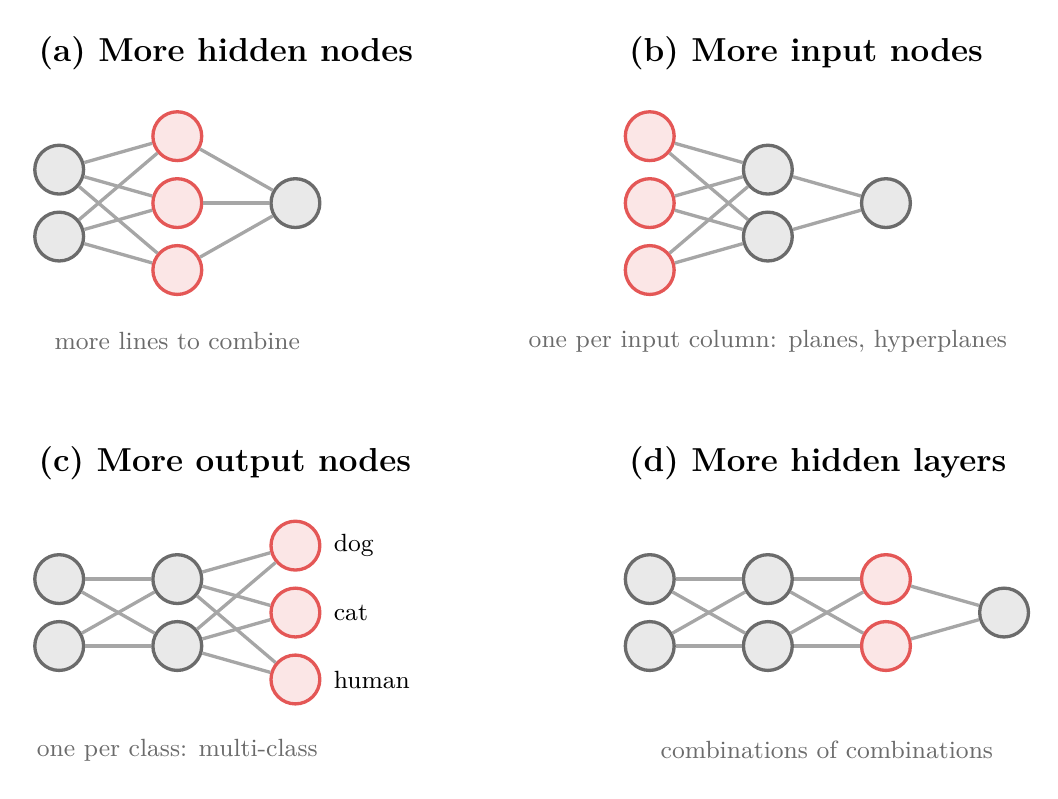
\begin{tikzpicture}[
  n/.style={circle, draw=#1, fill=#1!15, minimum size=0.62cm, line width=1.2pt},
  n/.default=cgrey]
  % helper: draw layer sizes as a fully connected net at origin (#1 list of sizes, #2 colour of the changed layer index)
  \newcommand{\net}[4]{% x0, y0, list of sizes, index of highlighted layer
    \foreach \s [count=\l from 0] in {#3} {
      \pgfmathsetmacro{\top}{(\s-1)/2*0.85}
      \foreach \k in {1,...,\s} {
        \pgfmathtruncatemacro{\hl}{\l==#4}
        \ifnum\hl=1 \node[n=cred] (L\l-\k) at (#1+\l*1.5, #2+\top-\k*0.85+0.85) {};
        \else \node[n] (L\l-\k) at (#1+\l*1.5, #2+\top-\k*0.85+0.85) {}; \fi
      }
    }
  }
  % (a) more hidden nodes: 2-3-1
  \net{0}{0}{2,3,1}{1}
  \foreach \i in {1,2} \foreach \j in {1,2,3} \draw[cgrey!60, on background layer] (L0-\i) -- (L1-\j);
  \foreach \i in {1,2,3} \draw[cgrey!60] (L1-\i) -- (L2-1);
  \node[font=\sffamily\large\bfseries, anchor=west] at (-0.4, 1.9) {(a) More hidden nodes};
  \node[note] at (1.5,-1.75) {more lines to combine};
  % (b) more input nodes: 3-2-1
  \begin{scope}[xshift=7.5cm]
  \net{0}{0}{3,2,1}{0}
  \foreach \i in {1,2,3} \foreach \j in {1,2} \draw[cgrey!60] (L0-\i) -- (L1-\j);
  \foreach \i in {1,2} \draw[cgrey!60] (L1-\i) -- (L2-1);
  \node[font=\sffamily\large\bfseries, anchor=west] at (-0.4, 1.9) {(b) More input nodes};
  \node[note] at (1.5,-1.75) {one per input column: planes, hyperplanes};
  \end{scope}
  % (c) more output nodes: 2-2-3
  \begin{scope}[yshift=-5.2cm]
  \net{0}{0}{2,2,3}{2}
  \foreach \i in {1,2} \foreach \j in {1,2} \draw[cgrey!60] (L0-\i) -- (L1-\j);
  \foreach \i in {1,2} \foreach \j in {1,2,3} \draw[cgrey!60] (L1-\i) -- (L2-\j);
  \node[anchor=west, font=\sffamily\small] at (3.35, 0.85) {dog};
  \node[anchor=west, font=\sffamily\small] at (3.35, 0) {cat};
  \node[anchor=west, font=\sffamily\small] at (3.35,-0.85) {human};
  \node[font=\sffamily\large\bfseries, anchor=west] at (-0.4, 1.9) {(c) More output nodes};
  \node[note] at (1.5,-1.75) {one per class: multi-class};
  \end{scope}
  % (d) more hidden layers: 2-2-2-1
  \begin{scope}[xshift=7.5cm, yshift=-5.2cm]
  \net{0}{0}{2,2,2,1}{2}
  \foreach \i in {1,2} \foreach \j in {1,2} {\draw[cgrey!60] (L0-\i) -- (L1-\j); \draw[cgrey!60] (L1-\i) -- (L2-\j);}
  \foreach \i in {1,2} \draw[cgrey!60] (L2-\i) -- (L3-1);
  \node[font=\sffamily\large\bfseries, anchor=west] at (-0.4, 1.9) {(d) More hidden layers};
  \node[note] at (2.25,-1.75) {combinations of combinations};
  \end{scope}
\end{tikzpicture}
\end{document}
